\documentclass[11pt, oneside]{article}   	% use "amsart" instead of "article" for AMSLaTeX format
\usepackage{geometry}                		% See geometry.pdf to learn the layout options. There are lots.
%\geometry{letterpaper}                   		% ... or a4paper or a5paper or ... 
\geometry{a4paper}                   		% ... or a4paper or a5paper or ... 
%\usepackage[parfill]{parskip}    		% Activate to begin paragraphs with an empty line rather than an indent
\usepackage{graphicx}				% Use pdf, png, jpg, or epsБ•√ with pdflatex; use eps in DVI mode
								% TeX will automatically convert eps --> pdf in pdflatex		
\usepackage{amssymb}
\usepackage[colorlinks]{hyperref}
\usepackage{booktabs}
\usepackage{amsmath}
\usepackage{multirow}% http://ctan.org/pkg/multirow
\usepackage{tablefootnote}
\usepackage{import}
\usepackage{subcaption}
\usepackage{caption}
\usepackage[format=hang,font=small,labelfont=bf]{caption}

\title{A quantitative assessment of the Hadoop framework for analysing massively parallel DNA sequencing data (Hadoop Or Not Hadoop)}
\author{Alexey Siretskiy,  Luca Pireddu, Ola Spjuth}
%\date{}							% Activate to display a given date or no date

\graphicspath { {./figures/fig1/} {./figures/fig2/} {./figures/fig9/} {./figures/fig5/}}

\begin{document}
\maketitle

\abstract{New high-throughput technologies such as massively parallel sequencing has transformed the life sciences into a data-intensive field. With increasing data volumes comes the necessity to analyse data in parallel using high-performance computing resources, but doing this effectively can be laborious and challenging. 
Hadoop, emerged in the last decade, is a framework that automatically distributes data and computation and has been shown to scale to thousands of nodes. We here report a quantitative comparison of Hadoop with regular high-performance computing resources for aligning short reads and calling variants for five datasets of different sizes up to 250\,Gigabases. In order to increase performance of existing software and obtain a better comparison we modified and wrote new analysis scripts. Observing the scaling relations we are able to draw conclusions about the perspectives of the approaches, leading to the conclusion that as data set sizes reach 100 Gigabases, the Hadoop-based pipelines become performance-competitive with a canonical high-performance cluster solution. As data sets in biological sequencing are sure to increase with time, Hadoop and similar frameworks are very interesting technologies that we envision will play a key role in future biological data analysis.
}


\section{Introduction}
\label{sectionI}
%The problem: dealing with BIG data
Since its inception, massively parallel DNA sequencing, also referred to as Next Generation Sequencing~(NGS) technology, has been an extremely bountiful source of data giving insight into the workings of biological machinery~\cite{metzker, marx}. Decreasing sequencing costs facilitates and promotes larger and larger studies with increasingly larger data sizes, and extracting useful information from these voluminous amounts of data is transforming biology into a data-intensive discipline.  As an example of the scale of the demands, consider that a single Illumina high-throughput sequencing run produces approximately 3\,TB of raw data in 10 days~\cite{illumina}.  Indeed, the Swedish UPPMAX\footnote{\url{uppmax.uu.se}} high-performance computing (HPC) center recently disclosed data showing that just in their sequencing context (most sequencing performed in Sweden) storage is being occupied at a rate of~1\,TB/day while the analyses are using over~1 million computing core-hours per month~\cite{lampa}. 

%Current practices: HPC systems
A common step of NGS data analysis consists of mapping short reads to a reference sequence and then finding the genetic variations specific to the sample. Most of the bioinformatic programs are written for the Linux operating system. Some of the most widespread tools \footnote{average number of invocations per month during 2013 at UPPMAX: Samtools~-- 30000, BWA~-- 25000, Bowtie~-- 5000} like BWA~\cite{bwa}, Bowtie~\cite{bowtie} and Samtools~\cite{samtools} are ``regular'' computer programs, not made up with distributed computing in mind; many others do not even have the native ability to use multiple cores on the same computer\footnote{Samtools  acquired this feature since v.0.1.19}. 

%Current practices: How to parallelize

The most common approach to speed up NGS tools is to parallelise within a compute node using shared memory parallelism~(OMP)~\cite{openmp}, but this approach is naturally limited by the number of cores per node which usually does not exceed~16.  For the tools which do not support the OMP natively, i.e. Samtools, variant calling can be parallelised by creating a separate process  for  each chromosome, or using GNU Parallel~\cite{gnuparallel} Linux utility.
Of great importance is that a multi-core approach does not improve the performance of operations that are limited by disk or network throughput, motivating to split  the dataset and  use multi-node parallelisation. Message Passing Interface~(MPI)~\cite{mpi1} is a common way to implement multi-node parallelisation, but writing efficient MPI-programs for hundreds of cores is a non-trivial task since all the threads synchronisation (or load balancing) has to be coded by a programmer and there are only a few existing solutions available for processing sequencing data~\cite{pmap, erne, gnumap}.

Another common way to introduce parallelisation in Linux systems is to use Bash scripting e.g. involve already existing utilities and cluster tools, split the data into chunks and process them on the separate nodes, and merging the results afterwards. This kind of solution benefits from both MPI and OMP and provides good performance, but the developments requires substantial expertise in order to be efficient, and the process is tightly coupled to the local computational cluster and network architectures and in many cases cannot be re-used in other settings.

%Introduce Hadoop, MR, and HDFS
%Properties of Hadoop and HDFS- data localization and programming model etc
The Map-Reduce~(MR) programming paradigm~\cite{hadoop} offers a compelling alternative for running task in a {\it massively} parallel way. This paradigm, however, shifts the focus from the best performance to scalability, suited for managing huge datasets of sizes up to several terabytes~\cite{lin2010}.
The prevalent open source implementation of Map-Reduce is Hadoop~\cite{hadoop,Hadoop:Guide}. 
The Hadoop~MR framework provides automatic distribution of computations over many nodes as well as automatic failure recovery (failure of individual jobs or computing nodes by storing multiple copies on different nodes), and automated collection of results~\cite{Hadoop:Guide}. Hadoop Distributed File System~(HDFS) is a complementary component that stores data by automatically distributing it over the entire cluster, writing data blocks onto the local disk of each node and therefore effectively moving the computation to the data and reducing network traffic. HDFS provides a storage system whose bandwidth and size scales with the number of nodes in the cluster~\cite{Sammer:2012}, which is very different from the properties of the usual HPC cluster network architecture. 

%Manuscript focus: When is Hadoop currently an appealing alternative
%Introduce what we did in the manuscript.
In this manuscript we focus on the question {\it if} and {\it when} Hadoop is an appealing alternative to the program tools generally found in~HPC centers for DNA-seq analysis. Since Hadoop is written in Java, which is slower than the standard~HPC programming languages like C or Fortran, we seek to estimate an average data size when it starts to be worthwhile to use Hadoop from a performance perspective. We use five datasets with short reads of different sizes, align them against the reference genome, and call the variances.
%From the algorithmic point of view we propose a modification of a code for a preprocessing stage for Crossbow in order to benefit fully from massively parallel nature of MR computations. 
For the classical HPC DNA-seq analysis programs we developed a set of bash scripts utilizing multiple nodes for short reads alignment and exploiting the network fully, thereby speeding up calculations.
The execution times for each dataset were collected and scaling relations were analysed to answer the question in focus.

The manuscript is structured as follows: In Section~II we briefly introduce the datasets, computational facilities, analysis pipelines design,  and the software used. Then, Section~III presents experimental results; first verifying that both HPC and Hadoop approaches extract the same mutation and then investigating the scaling relations in terms of data size and computing resources. The results are discussed in Section~IV, and conclusions in Section~V. Supplementary materials are provided in the corresponding section.



\section{Methods}
\label{sectionII}

\subsection{Datasets}
We used publicly available DNA-seq datasets~(I--III) and one synthetic dataset~(IV) for {\it A.thaliana}, the well known model plant, and one, (dataset~V) for two {\it H.sapiens} individuals (Table~\ref{table:datasets}). Data for datasets I-III and V were obtained using Illumina/(HiSeq) sequencing platforms. Further information about the datasets is provided in the Supplementary material section.


\begin{table}[htdp]
\small
\footnotesize
\caption{Datasets used}
\begin{center}
\begin{tabular}{|l|l|l|}
dataset &	organism &	size in Gbases\\
\hline
 I		&	{\it A.thaliana}	&	1.4	\\
 II	&	{\it A.thaliana}	&	7.0\\
  III	&	{\it A.thaliana}	&	30.0	\\
 IV	&{\it A.thaliana}, the artificial dataset created using Samtools package	&	100.0	\\
 V	&	{\it H.sapiens}, two individuals (GM12750 and GM12004), sample SRR499924		&	250.0\\

\end{tabular}
\end{center}
\label{table:datasets}
\normalsize
\end{table}%


\subsection{Analysis pipelines}
We constructed two pipelines for identifying SNPs from short read data, one based on Hadoop and one on regular HPC with a batch system (hereafter referred to as HPC). Our experiments then consisted of running the pipelines for the selected input dataset and measuring the wall-clock run time for each pipeline stage. All experiments were repeated several times and the results averaged to obtain a data point for the particular combination of data size and computational platform. Acknowledging that there are different approaches and software for conducting bioinformatic analysis for HPC (i.e. GATK~\cite{gatk}), we decided to create the  analysis pipeline as simple as possible to be able to pass the same stages on Hadoop and HPC:


\begin{enumerate}
\item HPC approach
\subitem Short read alignment: Bowtie~ver.~0.12.8
\subitem SNP calling: Samtool~ver.~0.1.19
\item Hadoop approach: Crossbow~\cite{crossbow}
\subitem Short read alignment: Bowtie~ver.~0.12.8
\subitem SNP calling: SOAPsnp~1.02~\cite{soapsnp}
\end{enumerate}


In the HPC pipeline, reads were aligned with Bowtie, followed by sorting the mapped reads and~SNP calling with Samtools. The Bowtie aligner natively implements~OMP meaning that with~8 cores on the same computer the result can be theoretically obtained 8 times faster than on a single core. Likewise, Samtools (as of version~0.1.19) also offers shared memory parallelism for several of its functions. Where available these features were used to improve the analysis speed. For the exact workflow used one can refer to the code repository created for this work~\cite{code_repo}.

The equivalent Hadoop-based pipeline was implemented with Crossbow. The input data and the indexed genome reference were copied to Hadoop's storage system~(HDFS) before starting the experiments. Crossbow implements a short pipeline that pre-processes the input data, transforming it into a format suitable for the alignment stage, and then continues to use Bowtie for alignment and SoapSNP to call SNPs.  Unfortunately Crossbow's preprocessor is not written in MR manner, and thus cannot be run in a massively parallel way. Due to this limitation, this basic step threatened to be the most time-consuming procedure in our test pipeline and bias our experiments. To overcome this bottleneck we substituted Crossbow's preprocessor with our own MR implementation, though sacrificing some generality\footnote{we assume that the FASTQ data are BZIP archived, and delivered to the storage accessible by Hadoop.}. To illustrate the benefits of this modification: For our 30-Gbase test dataset (approximately 45 GB of uncompressed FASTQ data) the preprocessing time shrunk from 3.3 hours to just under 2 minutes when run on 112 cores Hadoop cluster. The scripts for the preprocessing stage are publicly available~\cite{code_repo}.


\subsection{Computational resources}
To run the HPC analysis pipeline we used a computational cluster at UPPMAX, having nodes equipped with 4 dual-core CPUs. Data and reference genomes were stored on a parallel shared storage system. The Hadoop test platform was deployed on a private cloud at UPPMAX using the OpenNebula~\cite{opennebula} cloud manager. The cluster was set up with Cloudera Hadoop distribution version~2.0.0-cdh4.4.0~\cite{cloudera}. For details on computational resources, see Supplementary material.





\section{Results}
\label{sectionIII}

\subsection{Accuracy of pipelines}
Since our HPC and Hadoop approaches use different~SNP callers (Samtools and SOAPsnp correspondingly) we should not expect them to deliver perfectly matching SNPs lists, but still we expect them to capture and correctly identify the mutation. We tested the correctness just for the smallest dataset~I. The mutation $C\rightarrow T$ on chromosome 4 at position $16702262$ was successfully localized by both applications\cite{schneeberger}. [IS THIS REFERENCE CORRECT AND IN RIGHT PLACE?]

\subsection{Scalability of HPC and Hadoop approaches}
To demonstrate the scalability of  the HPC approach we collected running times for dataset~I as a function of the number of cores used (Table~\ref{table:hpctiming}).
As one can see the aligning process with the Bowtie scales linearly, but the SNP calling part is a definite bottleneck, showing almost no scaling at all.
For the given datasets (I--V) the timings for alignment against the corresponding genomes and SNP calling for  the HPC and Hadoop approaches were collected (Table~\ref{table:2}).

One of the attractive sides of using Hadoop is its almost linear scalability,~i.e. calculation time linearly depends on the size of the dataset\cite{crossbow,seal}, regardless the scaling nature of the underlying program (Samtools, Bowtie etc.). 
Figure~\ref{fig:fig1} shows the calculation time as a function of the dataset size for $p=56$ cores Hadoop cluster. Dataset V was excluded since it is for {\it H.sapiens}, which has more than 20 times larger genome than~{\it A.thaliana}.
To stress the linear nature of scaling, both sets of points were fit to linear polynomial using the least squares method.


\begin{table}[b]
\small
\caption{Calculation time for Dataset I executed on different  number of cores on a node of  HPC1 cluster. }
\begin{center}
\begin{tabular}{|c|c|c|c|}
$N$ cores	&\multicolumn{3}{c|}{timing, minutes}\\
\hline
	& aligning 	&	SNP calling\tablefootnote{We do not consider here special tricks how to parallelize the Samtools analysis by chromosome, as could be done, as exemplified here \url{http://www.biostars.org/p/48781/
}}	&	total \\
\hline
1	&	38	&	37		&	75 \\
2	&	19	&	36		&	55\\
4	&	10	&	36		&	46\\
8	&	5	&	36		&	41\\
\end{tabular}
\end{center}
\label{table:hpctiming}
\normalsize
\end{table}

\begin{table}[htdp]
\caption{Timings  (in minutes) for HPC and  Hadoop deployments for different dataset sizes.    Dataset is shown in brackets by roman numerals, ``f.r.'' stands for ``forward reads''.}
\begin{center}
\begin{tabular}{|l|c|c|c|c|c|c|c|}

data, Gbases&	1.4&	3.5&	7.0 	&15.0 	&30.0 	&100.0 	&250 	\\
			&	(I)			& (II, f.r.)	&	(II)		&(III, f.r.) &(III)&(IV) &(V)\\
\hline
Hadoop, 56 cores&--&	--	&39		&62	&108	&250&1125\\
\hline
%Hadoop, 56 cores, Shared~TM&	25	&	24	&40		&	70&	150	&410&\\
%\hline
%Hadoop, 56 cores, ``bare-metal''  &	36	&	41	&53  	&63	&	92& 380	&\\
%\hline
HPC1, 8 cores&	41&	96	&157	&307	&596	&1490&--\\
%\hline
%HPC2, 8 cores&72	&	&205	&&413&1765&\\
%\hline
%$F_{Hadoop}/F_{HPC1}$, Shared TM &	4.27		&1.75	&1.78	&	1.60	&	1.75	&	1.93&\\
%\hline
%$F_{Hadoop}/F_{HPC1}$, SSH TM &&		&1.74	&1.41	&1.28	&1.17	&\\
%\hline
%$F_{Hadoop}/F_{HPC2}$, ``bare-metal'' &&&&&&&\\

%data, 	& \multicolumn{2}{c|}{Hadoop, 56 cores}		  	&  HPC			&	\multicolumn{2}{c|}{$F_{Hadoop}/F_{HPC}$}\\
%Gbases 	&	 SSH~TM,	&	Shared~TM,	&	(8 cores), 	&	Shared TM	& 	SSH TM\\
%&  minutes& minutes&  minutes& &\\

\end{tabular}
\end{center}
\label{table:2}
\end{table}%




\begin{figure}
	% GNUPLOT: LaTeX picture with Postscript
\begingroup
  \makeatletter
  \providecommand\color[2][]{%
    \GenericError{(gnuplot) \space\space\space\@spaces}{%
      Package color not loaded in conjunction with
      terminal option `colourtext'%
    }{See the gnuplot documentation for explanation.%
    }{Either use 'blacktext' in gnuplot or load the package
      color.sty in LaTeX.}%
    \renewcommand\color[2][]{}%
  }%
  \providecommand\includegraphics[2][]{%
    \GenericError{(gnuplot) \space\space\space\@spaces}{%
      Package graphicx or graphics not loaded%
    }{See the gnuplot documentation for explanation.%
    }{The gnuplot epslatex terminal needs graphicx.sty or graphics.sty.}%
    \renewcommand\includegraphics[2][]{}%
  }%
  \providecommand\rotatebox[2]{#2}%
  \@ifundefined{ifGPcolor}{%
    \newif\ifGPcolor
    \GPcolorfalse
  }{}%
  \@ifundefined{ifGPblacktext}{%
    \newif\ifGPblacktext
    \GPblacktexttrue
  }{}%
  % define a \g@addto@macro without @ in the name:
  \let\gplgaddtomacro\g@addto@macro
  % define empty templates for all commands taking text:
  \gdef\gplbacktext{}%
  \gdef\gplfronttext{}%
  \makeatother
  \ifGPblacktext
    % no textcolor at all
    \def\colorrgb#1{}%
    \def\colorgray#1{}%
  \else
    % gray or color?
    \ifGPcolor
      \def\colorrgb#1{\color[rgb]{#1}}%
      \def\colorgray#1{\color[gray]{#1}}%
      \expandafter\def\csname LTw\endcsname{\color{white}}%
      \expandafter\def\csname LTb\endcsname{\color{black}}%
      \expandafter\def\csname LTa\endcsname{\color{black}}%
      \expandafter\def\csname LT0\endcsname{\color[rgb]{1,0,0}}%
      \expandafter\def\csname LT1\endcsname{\color[rgb]{0,1,0}}%
      \expandafter\def\csname LT2\endcsname{\color[rgb]{0,0,1}}%
      \expandafter\def\csname LT3\endcsname{\color[rgb]{1,0,1}}%
      \expandafter\def\csname LT4\endcsname{\color[rgb]{0,1,1}}%
      \expandafter\def\csname LT5\endcsname{\color[rgb]{1,1,0}}%
      \expandafter\def\csname LT6\endcsname{\color[rgb]{0,0,0}}%
      \expandafter\def\csname LT7\endcsname{\color[rgb]{1,0.3,0}}%
      \expandafter\def\csname LT8\endcsname{\color[rgb]{0.5,0.5,0.5}}%
    \else
      % gray
      \def\colorrgb#1{\color{black}}%
      \def\colorgray#1{\color[gray]{#1}}%
      \expandafter\def\csname LTw\endcsname{\color{white}}%
      \expandafter\def\csname LTb\endcsname{\color{black}}%
      \expandafter\def\csname LTa\endcsname{\color{black}}%
      \expandafter\def\csname LT0\endcsname{\color{black}}%
      \expandafter\def\csname LT1\endcsname{\color{black}}%
      \expandafter\def\csname LT2\endcsname{\color{black}}%
      \expandafter\def\csname LT3\endcsname{\color{black}}%
      \expandafter\def\csname LT4\endcsname{\color{black}}%
      \expandafter\def\csname LT5\endcsname{\color{black}}%
      \expandafter\def\csname LT6\endcsname{\color{black}}%
      \expandafter\def\csname LT7\endcsname{\color{black}}%
      \expandafter\def\csname LT8\endcsname{\color{black}}%
    \fi
  \fi
  \setlength{\unitlength}{0.0500bp}%
  \begin{picture}(8502.00,5668.00)%
    \gplgaddtomacro\gplbacktext{%
      \csname LTb\endcsname%
      \put(946,704){\makebox(0,0)[r]{\strut{} 0}}%
      \csname LTb\endcsname%
      \put(946,1421){\makebox(0,0)[r]{\strut{} 50}}%
      \csname LTb\endcsname%
      \put(946,2138){\makebox(0,0)[r]{\strut{} 100}}%
      \csname LTb\endcsname%
      \put(946,2856){\makebox(0,0)[r]{\strut{} 150}}%
      \csname LTb\endcsname%
      \put(946,3573){\makebox(0,0)[r]{\strut{} 200}}%
      \csname LTb\endcsname%
      \put(946,4290){\makebox(0,0)[r]{\strut{} 250}}%
      \csname LTb\endcsname%
      \put(946,5007){\makebox(0,0)[r]{\strut{} 300}}%
      \csname LTb\endcsname%
      \put(1078,484){\makebox(0,0){\strut{} 0}}%
      \csname LTb\endcsname%
      \put(1717,484){\makebox(0,0){\strut{} 10}}%
      \csname LTb\endcsname%
      \put(2356,484){\makebox(0,0){\strut{} 20}}%
      \csname LTb\endcsname%
      \put(2994,484){\makebox(0,0){\strut{} 30}}%
      \csname LTb\endcsname%
      \put(3633,484){\makebox(0,0){\strut{} 40}}%
      \csname LTb\endcsname%
      \put(4272,484){\makebox(0,0){\strut{} 50}}%
      \csname LTb\endcsname%
      \put(4911,484){\makebox(0,0){\strut{} 60}}%
      \csname LTb\endcsname%
      \put(5550,484){\makebox(0,0){\strut{} 70}}%
      \csname LTb\endcsname%
      \put(6189,484){\makebox(0,0){\strut{} 80}}%
      \csname LTb\endcsname%
      \put(6827,484){\makebox(0,0){\strut{} 90}}%
      \csname LTb\endcsname%
      \put(7466,484){\makebox(0,0){\strut{} 100}}%
      \csname LTb\endcsname%
      \put(8105,484){\makebox(0,0){\strut{} 110}}%
      \put(176,2855){\rotatebox{-270}{\makebox(0,0){\strut{}calculation time, minutes}}}%
      \put(4591,154){\makebox(0,0){\strut{}dataset size, Gbases}}%
      \put(4591,5337){\makebox(0,0){\strut{}Figure 1}}%
    }%
    \gplgaddtomacro\gplfronttext{%
      \csname LTb\endcsname%
      \put(3158,4834){\makebox(0,0)[l]{\strut{}Hadoop}}%
      \csname LTb\endcsname%
      \put(1168,776){\makebox(0,0){\strut{}}}%
      \put(1302,776){\makebox(0,0){\strut{}}}%
      \put(1525,977){\makebox(0,0){\strut{}datasetII}}%
      \put(2037,1306){\makebox(0,0){\strut{}}}%
      \put(2995,1995){\makebox(0,0){\strut{}datasetIII}}%
      \put(7467,4003){\makebox(0,0){\strut{}datasetIV}}%
      \csname LTb\endcsname%
      \put(3158,4614){\makebox(0,0)[l]{\strut{}Linear fit for the Hadoop data}}%
    }%
    \gplbacktext
    \put(0,0){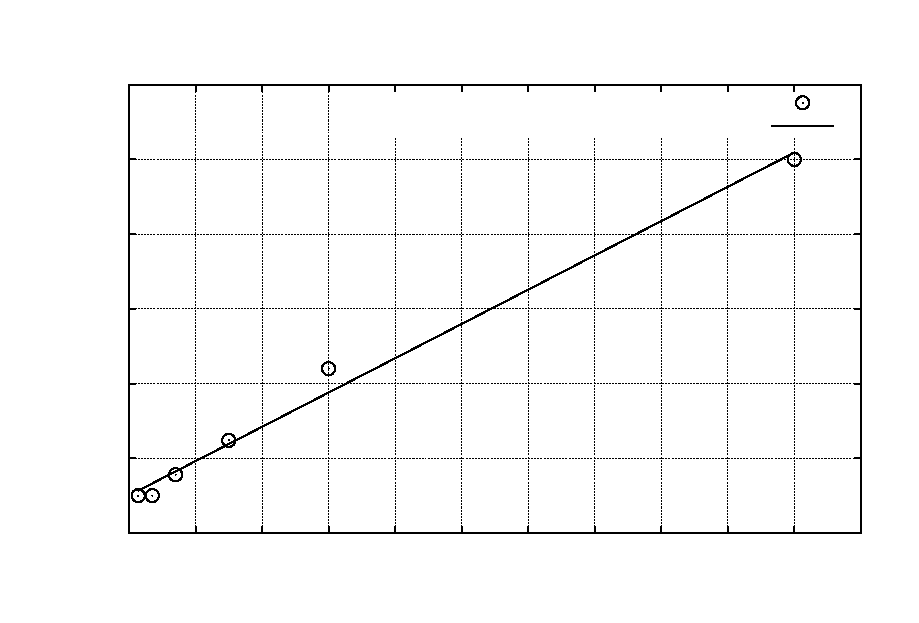
\includegraphics{fig1}}%
    \gplfronttext
  \end{picture}%
\endgroup

	\caption{Calculation time depending on the dataset size for fixed size~($p=56$ cores) of Hadoop cluster on the private Cloud. The linear fit based on least squares method are provided, revealing almost linear scaling.}
	\label{fig:fig1}
\end{figure}


\subsection{Comparing Hadoop and HPC efficiency for different dataset sizes}
Hadoop initially was designed to digest huge datasets\cite{hadoop,lin2010}. One can propose then that the larger the dataset is, the more suitable Hadoop becomes compare to the HPC approach. In order to compare the ''suitability'' for different types of calculation platforms (Hadoop and HPC) each being run on different amount of cores, we constructed the following function:
$$F=T_{p}\times p,$$ 
where~$T_{p}$ is the calculation time on~$p$ cores.
Using the data from Table~\ref{table:2},  we plot the ratio $F_{Hadoop}/F_{HPC}$, keeping in mind that the closer the ratio to the unity, the closer Hadoop's efficiency is to that of the HPC approach.


\begin{figure}
	% GNUPLOT: LaTeX picture with Postscript
\begingroup
  \makeatletter
  \providecommand\color[2][]{%
    \GenericError{(gnuplot) \space\space\space\@spaces}{%
      Package color not loaded in conjunction with
      terminal option `colourtext'%
    }{See the gnuplot documentation for explanation.%
    }{Either use 'blacktext' in gnuplot or load the package
      color.sty in LaTeX.}%
    \renewcommand\color[2][]{}%
  }%
  \providecommand\includegraphics[2][]{%
    \GenericError{(gnuplot) \space\space\space\@spaces}{%
      Package graphicx or graphics not loaded%
    }{See the gnuplot documentation for explanation.%
    }{The gnuplot epslatex terminal needs graphicx.sty or graphics.sty.}%
    \renewcommand\includegraphics[2][]{}%
  }%
  \providecommand\rotatebox[2]{#2}%
  \@ifundefined{ifGPcolor}{%
    \newif\ifGPcolor
    \GPcolorfalse
  }{}%
  \@ifundefined{ifGPblacktext}{%
    \newif\ifGPblacktext
    \GPblacktexttrue
  }{}%
  % define a \g@addto@macro without @ in the name:
  \let\gplgaddtomacro\g@addto@macro
  % define empty templates for all commands taking text:
  \gdef\gplbacktext{}%
  \gdef\gplfronttext{}%
  \makeatother
  \ifGPblacktext
    % no textcolor at all
    \def\colorrgb#1{}%
    \def\colorgray#1{}%
  \else
    % gray or color?
    \ifGPcolor
      \def\colorrgb#1{\color[rgb]{#1}}%
      \def\colorgray#1{\color[gray]{#1}}%
      \expandafter\def\csname LTw\endcsname{\color{white}}%
      \expandafter\def\csname LTb\endcsname{\color{black}}%
      \expandafter\def\csname LTa\endcsname{\color{black}}%
      \expandafter\def\csname LT0\endcsname{\color[rgb]{1,0,0}}%
      \expandafter\def\csname LT1\endcsname{\color[rgb]{0,1,0}}%
      \expandafter\def\csname LT2\endcsname{\color[rgb]{0,0,1}}%
      \expandafter\def\csname LT3\endcsname{\color[rgb]{1,0,1}}%
      \expandafter\def\csname LT4\endcsname{\color[rgb]{0,1,1}}%
      \expandafter\def\csname LT5\endcsname{\color[rgb]{1,1,0}}%
      \expandafter\def\csname LT6\endcsname{\color[rgb]{0,0,0}}%
      \expandafter\def\csname LT7\endcsname{\color[rgb]{1,0.3,0}}%
      \expandafter\def\csname LT8\endcsname{\color[rgb]{0.5,0.5,0.5}}%
    \else
      % gray
      \def\colorrgb#1{\color{black}}%
      \def\colorgray#1{\color[gray]{#1}}%
      \expandafter\def\csname LTw\endcsname{\color{white}}%
      \expandafter\def\csname LTb\endcsname{\color{black}}%
      \expandafter\def\csname LTa\endcsname{\color{black}}%
      \expandafter\def\csname LT0\endcsname{\color{black}}%
      \expandafter\def\csname LT1\endcsname{\color{black}}%
      \expandafter\def\csname LT2\endcsname{\color{black}}%
      \expandafter\def\csname LT3\endcsname{\color{black}}%
      \expandafter\def\csname LT4\endcsname{\color{black}}%
      \expandafter\def\csname LT5\endcsname{\color{black}}%
      \expandafter\def\csname LT6\endcsname{\color{black}}%
      \expandafter\def\csname LT7\endcsname{\color{black}}%
      \expandafter\def\csname LT8\endcsname{\color{black}}%
    \fi
  \fi
  \setlength{\unitlength}{0.0500bp}%
  \begin{picture}(8502.00,5668.00)%
    \gplgaddtomacro\gplbacktext{%
      \csname LTb\endcsname%
      \put(946,704){\makebox(0,0)[r]{\strut{} 1.1}}%
      \csname LTb\endcsname%
      \put(946,1319){\makebox(0,0)[r]{\strut{} 1.2}}%
      \csname LTb\endcsname%
      \put(946,1933){\makebox(0,0)[r]{\strut{} 1.3}}%
      \csname LTb\endcsname%
      \put(946,2548){\makebox(0,0)[r]{\strut{} 1.4}}%
      \csname LTb\endcsname%
      \put(946,3163){\makebox(0,0)[r]{\strut{} 1.5}}%
      \csname LTb\endcsname%
      \put(946,3778){\makebox(0,0)[r]{\strut{} 1.6}}%
      \csname LTb\endcsname%
      \put(946,4392){\makebox(0,0)[r]{\strut{} 1.7}}%
      \csname LTb\endcsname%
      \put(946,5007){\makebox(0,0)[r]{\strut{} 1.8}}%
      \csname LTb\endcsname%
      \put(1078,484){\makebox(0,0){\strut{} 0}}%
      \csname LTb\endcsname%
      \put(1956,484){\makebox(0,0){\strut{} 0.02}}%
      \csname LTb\endcsname%
      \put(2835,484){\makebox(0,0){\strut{} 0.04}}%
      \csname LTb\endcsname%
      \put(3713,484){\makebox(0,0){\strut{} 0.06}}%
      \csname LTb\endcsname%
      \put(4592,484){\makebox(0,0){\strut{} 0.08}}%
      \csname LTb\endcsname%
      \put(5470,484){\makebox(0,0){\strut{} 0.1}}%
      \csname LTb\endcsname%
      \put(6348,484){\makebox(0,0){\strut{} 0.12}}%
      \csname LTb\endcsname%
      \put(7227,484){\makebox(0,0){\strut{} 0.14}}%
      \csname LTb\endcsname%
      \put(8105,484){\makebox(0,0){\strut{} 0.16}}%
      \put(176,2855){\rotatebox{-270}{\makebox(0,0){\strut{}ratio of $F_{Hadoop}/F_{HPC}$}}}%
      \put(4591,154){\makebox(0,0){\strut{}reciprocal dataset size, 1/Gbases}}%
      \put(4591,5337){\makebox(0,0){\strut{}Figure 2}}%
    }%
    \gplgaddtomacro\gplfronttext{%
      \csname LTb\endcsname%
      \put(7578,4423){\makebox(0,0){\strut{}datasetI}}%
      \put(4240,2394){\makebox(0,0){\strut{}datasetII}}%
      \put(2747,1595){\makebox(0,0){\strut{}datasetIII}}%
      \put(1737,919){\makebox(0,0){\strut{}datasetIV}}%
      \csname LTb\endcsname%
      \put(1310,4834){\makebox(0,0)[l]{\strut{}least-squares fit to $y=aX+b$ for the data with  $b=1.13$}}%
    }%
    \gplbacktext
    \put(0,0){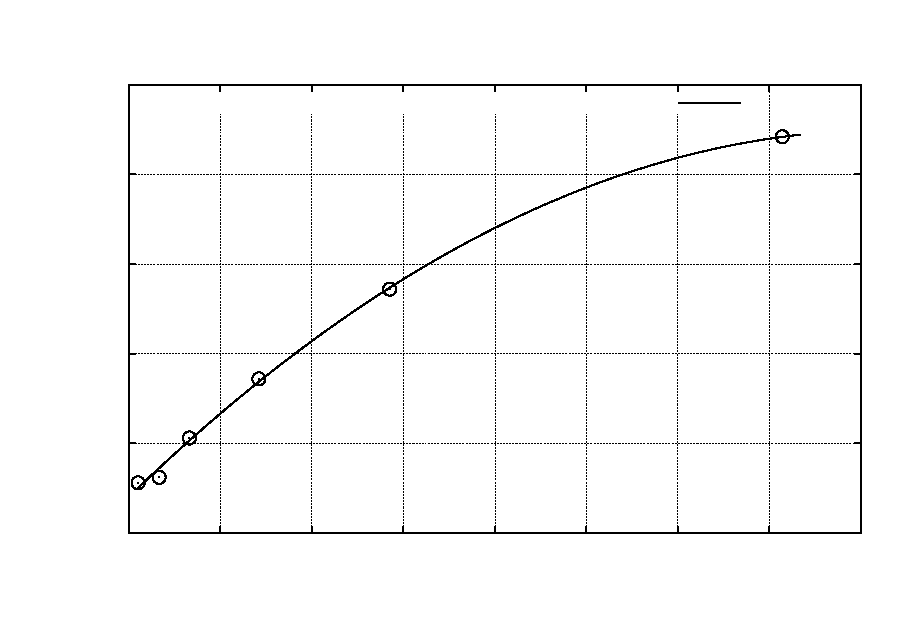
\includegraphics{fig2}}%
    \gplfronttext
  \end{picture}%
\endgroup

	\caption{The ratio of the~$F_{Hadoop}/F_{HPC}$ as a function of a reciprocal dataset size in Gigabases.  Calculations were carried out for~$p=56$ and $p=8$ cores for Hadoop and HPC1 correspondingly.
The points are fit in a line using least-squares method, what makes  possible to make some careful predictions for the case of the {\it infinite} dataset size.}
	\label{fig:fig2}
\end{figure}


The curve  in~Figure~\ref{fig:fig2} is plotted for~$p=56$ cores Hadoop cluster and an HPC node ($p=8$), and displays the ratio~$F_{Hadoop}/F_{HPC}$ as a function of the reciprocal dataset size. The extrapolation to the zero of the~$X$-axis tells the ratio for the hypothetical infinite dataset. As one can see, the Hadoop approach becomes more  and more effective compared to the HPC scenario as the data is larger. With  the linear extrapolation  the ratio reads~$1.13\pm0.01$, meaning that Hadoop running even  in the virtualized environment of a private cloud, is competitive with  the HPC approach which is being run on ''bare metal''  for the datasets greater than $100$\,Gbases (IV), which is a usual size for human genome sequencing giving the average sequencing depth of  about~$30x$.



 \subsection{Comparing the network communication efficiency for Hadoop and HPC approaches }
Network communication model for Hadoop has a major difference from the usual HPC cluster network architecture ($n$-tier tree) with the NAS or NFS attached storages. Namely, the effective bandwidth of the Hadoop network increases with the cluster size to increase~\cite{Sammer:2012}, opposite to that of the HPC network, where the cluster grows results in network saturation and performance depletion.
We provide a comparison how HPC and Hadoop  network communication costs depend on the number of nodes involved, for a fixed dataset size, dataset~IV.
 
Due to the fact of trivial parallelisation of the alignment process~-- the read-pairs are independent of each other, and can be aligned independently~-- one could try to involve more computation resources, i.e. split the initial data into chunks to proceed them independently.
Reducing the size of each data chunk reduces the aligner  job,~$T_{mapping}$, but at the same time, the more chunks almost {\it simultaneously} have to travel through the network, potentially causing traffic jams, therefore increasing the communication costs,~$T_{comm}$.

There are several program packages for short reads alignment designed with the MPI support~\cite{pmap, gnumap}. Authors report almost linear scaling up to 32 nodes for pair-ended reads\footnote{\url{http://bmi.osu.edu/hpc/slides/Bozdag10-HiCOMB.pdf}, \url{http://dna.cs.byu.edu/gnumap/HICOMB_Presentation.pdf}}. However,  i.e. Pmap package had been proved to function poorly on UPPMAX cluster for  datasets larger than 20 Gbases, raising  memory exceptions.
We wrote custom state-of-art bash script involving existing Unix utilities~\cite{repo} to use the  HPC2 cluster network as efficiently as possible,  and compared the network performance with the {\it standard} Hadoop HDFS approach.

We separated the mapping time~$T_{mapping}$ and the  communication time~ $T_{comm}$, and plot their ratio~$T_{mapping}/T_{comm}$ as a function of a reciprocal number of nodes~$1/N$. 
Such kind of measure is applicable to both HPC and Hadoop, however, the~$T_{comm}$ carries a different sense in both cases. For Hadoop the short reads in FASTQ format have to be preprocessed (involving nodes communication~$T_{comm}$) to  able to be run in the MR-fashion, while the data locality will be automatically achieved during the data  ingestion into the HDFS. 
We rewrote the code for the preprocessing stage for the Crossbow to make it suitable for MR-style parallelisation.
For the HPC approach, the~$T_{comm}$ involves the chunks travel from the sequencer delivery location to the local node scratches, where the actual mapping happens, and the travel of the aligned SAM files back to the delivery location over the network. 

Figure~\ref{fig:fig3} shows the~$T_{mapping}/T_{comm}$ ratio as a function of the reciprocal number of nodes~$1/N$ for Hadoop and HPC approaches. In its turn, the HPC approach is presented in two versions, which are based on a bit different strategies of the resource allocation.  

Lets start from description of the Hadoop results, filled circles. One can see that the ratio~$T_{mapping}/T_{comm}$ reveals very weak dependency in a wide range of number of nodes~$N$: from 4 up to 40. It is known  that the Bowtie, used for mapping, provides a linear scaling between the mapping time and the dataset chunk size~$D$:~$T_{mapping}\propto  D\propto 1/N$, see~\cite{bowtie}, and Figure 1. Since the ratio~$T_{mapping}/T_{comm}\approx const$, one can conclude that the~$T_{comm}\propto 1/N$, meaning that the more nodes are involved, the faster the communication in the preprocessing stage is. 

Lets now consider the curves for HPC2. The strategy named HPC SLURM\footnote{Simple Linux Utility for Resource Management} is as follows: the data from the delivery location is being split into chunks in {\it parallel}, which are  {\it simultaneously} being pushed  to the local scratches of the nodes, allocated by SLURM  (open circles). One can see two distinct linear stretches, each with different tangent. One stretch is for the range from 4 to about 12 nodes the, and the another is from 12 up to 60. The former, horizontal stretch, is explained as for Hadoop~-- the more nodes is being involved the faster the chunks are being distributed. The latter stretch with the positive slope could be explained as follows: in the region of about 12 nodes the network becomes saturated\footnote{The used storage at UPPMAX   is a set of RAIDs (Redundant Array of Inexpensive Disks) with data {\it striping}, providing up to $80$Gbit/sec of outcoming traffic} and unable to pass more data in a time unit, while the mapping time is still proportional to the chunk size:~$T_{comm}\approx const, T_{mapping}\propto D\propto 1/N \rightarrow T_{mapping}/T_{comm}\propto 1/N$, i.e. a linear dependency, which one can observe on the plot. 
The transition area between two modes~-- saturated and unsaturated~-- has the next origin: each HDD on the local node can write the data at a speed about 100MB/sec\,$\approx$\,1Gbit/sec, i.e.~10 nodes will consume the data with the rate of~10Gbit/sec, what is the limiting speed for the standard 10Gbit Ethernet cable connecting the cluster's rack with the switch. The nodes are being allocated  on the same rack, what is the default SLURM behaviour, therefore the caption reads~``HPC SLURM''. 

The scalability can be improved by overriding the default behaviour of the SLURM and allocating the nodes not from the same rack, but randomly from all available racks, ``HPC random'', (open squares in Figure~\ref{fig:fig3}). Allocating the nodes on random racks allows one to engage more nodes without network saturation. For our cluster we could go up to 30-35 nodes with perfect linear scaling. For the most resources been used (58 nodes) the deviation from a linear speed-up is~$\approx 7\%$ i.e. $5.50$ minutes against the ideal $5.14$, see Table~\ref{table:4}  for the data.



\begin{figure}
	\small
	% GNUPLOT: LaTeX picture with Postscript
\begingroup
  \makeatletter
  \providecommand\color[2][]{%
    \GenericError{(gnuplot) \space\space\space\@spaces}{%
      Package color not loaded in conjunction with
      terminal option `colourtext'%
    }{See the gnuplot documentation for explanation.%
    }{Either use 'blacktext' in gnuplot or load the package
      color.sty in LaTeX.}%
    \renewcommand\color[2][]{}%
  }%
  \providecommand\includegraphics[2][]{%
    \GenericError{(gnuplot) \space\space\space\@spaces}{%
      Package graphicx or graphics not loaded%
    }{See the gnuplot documentation for explanation.%
    }{The gnuplot epslatex terminal needs graphicx.sty or graphics.sty.}%
    \renewcommand\includegraphics[2][]{}%
  }%
  \providecommand\rotatebox[2]{#2}%
  \@ifundefined{ifGPcolor}{%
    \newif\ifGPcolor
    \GPcolorfalse
  }{}%
  \@ifundefined{ifGPblacktext}{%
    \newif\ifGPblacktext
    \GPblacktexttrue
  }{}%
  % define a \g@addto@macro without @ in the name:
  \let\gplgaddtomacro\g@addto@macro
  % define empty templates for all commands taking text:
  \gdef\gplbacktext{}%
  \gdef\gplfronttext{}%
  \makeatother
  \ifGPblacktext
    % no textcolor at all
    \def\colorrgb#1{}%
    \def\colorgray#1{}%
  \else
    % gray or color?
    \ifGPcolor
      \def\colorrgb#1{\color[rgb]{#1}}%
      \def\colorgray#1{\color[gray]{#1}}%
      \expandafter\def\csname LTw\endcsname{\color{white}}%
      \expandafter\def\csname LTb\endcsname{\color{black}}%
      \expandafter\def\csname LTa\endcsname{\color{black}}%
      \expandafter\def\csname LT0\endcsname{\color[rgb]{1,0,0}}%
      \expandafter\def\csname LT1\endcsname{\color[rgb]{0,1,0}}%
      \expandafter\def\csname LT2\endcsname{\color[rgb]{0,0,1}}%
      \expandafter\def\csname LT3\endcsname{\color[rgb]{1,0,1}}%
      \expandafter\def\csname LT4\endcsname{\color[rgb]{0,1,1}}%
      \expandafter\def\csname LT5\endcsname{\color[rgb]{1,1,0}}%
      \expandafter\def\csname LT6\endcsname{\color[rgb]{0,0,0}}%
      \expandafter\def\csname LT7\endcsname{\color[rgb]{1,0.3,0}}%
      \expandafter\def\csname LT8\endcsname{\color[rgb]{0.5,0.5,0.5}}%
    \else
      % gray
      \def\colorrgb#1{\color{black}}%
      \def\colorgray#1{\color[gray]{#1}}%
      \expandafter\def\csname LTw\endcsname{\color{white}}%
      \expandafter\def\csname LTb\endcsname{\color{black}}%
      \expandafter\def\csname LTa\endcsname{\color{black}}%
      \expandafter\def\csname LT0\endcsname{\color{black}}%
      \expandafter\def\csname LT1\endcsname{\color{black}}%
      \expandafter\def\csname LT2\endcsname{\color{black}}%
      \expandafter\def\csname LT3\endcsname{\color{black}}%
      \expandafter\def\csname LT4\endcsname{\color{black}}%
      \expandafter\def\csname LT5\endcsname{\color{black}}%
      \expandafter\def\csname LT6\endcsname{\color{black}}%
      \expandafter\def\csname LT7\endcsname{\color{black}}%
      \expandafter\def\csname LT8\endcsname{\color{black}}%
    \fi
  \fi
  \setlength{\unitlength}{0.0500bp}%
  \begin{picture}(8502.00,5668.00)%
    \gplgaddtomacro\gplbacktext{%
      \csname LTb\endcsname%
      \put(946,704){\makebox(0,0)[r]{\strut{} 0}}%
      \put(946,1242){\makebox(0,0)[r]{\strut{} 0.5}}%
      \put(946,1780){\makebox(0,0)[r]{\strut{} 1}}%
      \put(946,2318){\makebox(0,0)[r]{\strut{} 1.5}}%
      \put(946,2856){\makebox(0,0)[r]{\strut{} 2}}%
      \put(946,3393){\makebox(0,0)[r]{\strut{} 2.5}}%
      \put(946,3931){\makebox(0,0)[r]{\strut{} 3}}%
      \put(946,4469){\makebox(0,0)[r]{\strut{} 3.5}}%
      \put(946,5007){\makebox(0,0)[r]{\strut{} 4}}%
      \put(1078,484){\makebox(0,0){\strut{} 0}}%
      \put(2483,484){\makebox(0,0){\strut{} 0.05}}%
      \put(3889,484){\makebox(0,0){\strut{} 0.1}}%
      \put(5294,484){\makebox(0,0){\strut{} 0.15}}%
      \put(6700,484){\makebox(0,0){\strut{} 0.2}}%
      \put(8105,484){\makebox(0,0){\strut{} 0.25}}%
      \put(176,2855){\rotatebox{-270}{\makebox(0,0){\strut{}$T_{mapping}/T_{comm}$}}}%
      \put(4591,154){\makebox(0,0){\strut{}reciprocal number of nodes, $1/N$}}%
      \put(4591,5337){\makebox(0,0){\strut{}Ratios of the  short reads mapping time per node to the communication  time}}%
    }%
    \gplgaddtomacro\gplfronttext{%
      \csname LTb\endcsname%
      \put(7118,1977){\makebox(0,0)[r]{\strut{}HPC SLURM}}%
      \csname LTb\endcsname%
      \put(7118,1757){\makebox(0,0)[r]{\strut{}Hadoop}}%
      \csname LTb\endcsname%
      \put(7118,1537){\makebox(0,0)[r]{\strut{}HPC random}}%
      \csname LTb\endcsname%
      \put(7118,1317){\makebox(0,0)[r]{\strut{}linear fit for Hadoop }}%
      \csname LTb\endcsname%
      \put(7118,1097){\makebox(0,0)[r]{\strut{}linear fit for HPC SLURM}}%
      \csname LTb\endcsname%
      \put(7118,877){\makebox(0,0)[r]{\strut{}linear fit for HPC random}}%
    }%
    \gplbacktext
    \put(0,0){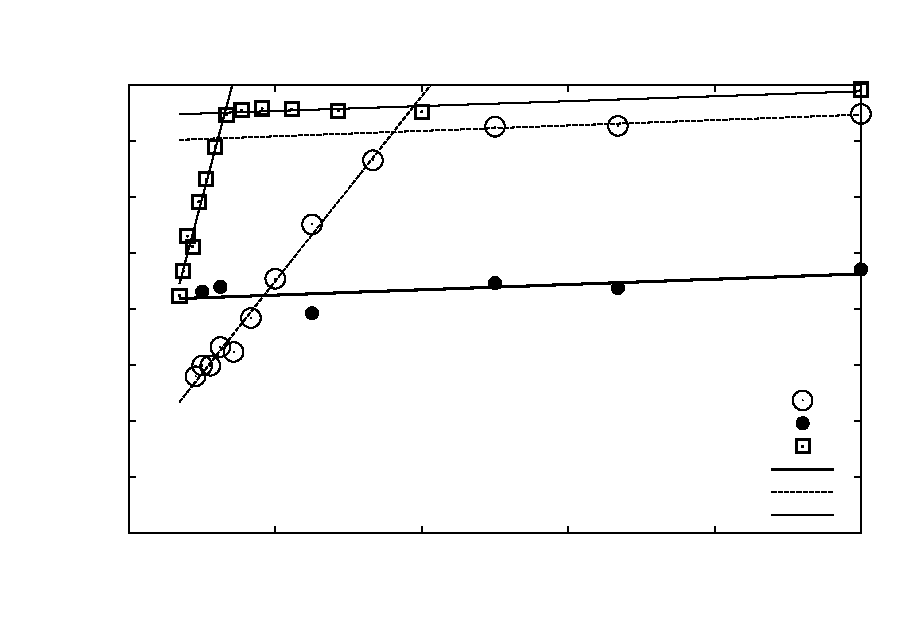
\includegraphics{fig3}}%
    \gplfronttext
  \end{picture}%
\endgroup

	\normalsize
	\caption{Ratios of the mapping time~$T_{mapping}$ to the communication costs~$T_{comm}$ for HPC2 and Hadoop clusters for Dataset IV as a function of reciprocal cluster size $1/N$. Two HPC scenarios are shown as ``HPC SLURM'' and ``HPC random'', which correspond to standard SLURM behaviour and a modified one, where nodes are being allocated from random racks.
%One  can see the differences in the Hadoop and HPC communication patterns: for Hadoop the ratio is almost constant, while for HPC cluster there are two defined regions.
%The first one resembles to that of Hadoop, and corresponds to the case then the communication in the cluster is not a bottleneck. 
%The second one shows the regime corresponding to the case of saturation of the network, resulting in traffic jams: data distibution time~$T_{comm}$ stops to scale 
%linearly to the reciprocal cluster size, and becomes more of less a constant, while the mapping time continues to satisfy~$T_{mapping}\propto 1/N$.
Linear fit  done with the least-squares method.}
	\label{fig:fig3}
\end{figure}

The threshold number of nodes in this strategy~($\approx35$) is driven by the saturating the uplink cable with the  throughput of~50Gbit/sec. 
The proposed strategies aimed to gain the maximum from the existing resources show, that even properly adjusted and tuned, HPC approach sooner of later starts to suffer from the network saturation.  


\begin{table}[htdp]
\caption{Timings  for mapping, and the ratio~$T_{mapping}/T_{comm}$  for HPC2 and  Hadoop clusters for Dataset IV.
For ``HPC random'' approach data chunks have to be copied to the local scratches first, and  the alignments (SAM files) copied back, while Hadoop keeps all the data inside HDFS. Hadoop needs to preprocess reads before the actual alignment stage, in order  to be able to operate in a MR manner, also resulting in  ``communication costs''. Note that each HPC node has 16 cores, while each Hadoop node has 7 (one core is dedicated to run the virtual machine).}
\begin{center}
\begin{tabular}{|c|c|c|c|c|c|}
 \multicolumn{3}{|c|}{Hadoop} & \multicolumn{3}{c|}{ HPC random} \\
 \hline		


Number nodes	&Mapping time,	&$\frac{T_{mapping}}{T_{comm}}$	&Number  nodes	&Mapping time,	&$\frac{T_{mapping}}{T_{comm}}$\\
(cores)					&minutes		&							&(cores)			&minutes&\\
\hline
4(28)	&293.5	&2.33	&4(64)	&74.4	&3.89\\
6(42)	&189.8	&2.19	&10(160)	&32.4	&3.76\\
8(56)	&136.0	&2.23	&14(224)	&22.7	&3.77\\
16(112)	&70.3	&1.96	&18(288)	&17.9	&3.78\\
32(224)	&39.3	&2.20	&22(352)	&14.5	&3.79\\
40(280)	&32.5	&2.15	&26(416)	&12.3	&3.77\\
			&&&30(480)	&10.7	&3.73\\
			&&&34(544)	&9.5	&3.45\\
			&&&38(608)	&8.5	&3.16\\
			&&&42(672)	&7.6	&2.96\\
			&&&46(736)	&7.0	&2.55\\
			&&&50(800)	&6.4	&2.65\\
			&&&54(864)	&5.9	&2.34\\
			&&&58(928)	&5.5	&2.12\\

\end{tabular}
\end{center}
\label{table:4}
\end{table}%
 At the same time, the HDFS keeps data locality, aiming to reduce the amount of communications, resulting less data move and, therefore, better scalability.
Our Hadoop-in-the-Cloud cluster has no more~($\approx 40$) free nodes to continue to investigate the scaling as in plot at Figure~\ref{fig:fig3}, but we do not expect any significant deviations, since the exposed behaviour is a generic for Hadoop with HDFS.


\subsection{Usability aspects}
\label{subsectionIV_2}

At the present moment a popular way to steer the bioinformatic pipelines on the HPC resources  is to use Galaxy\cite{galaxy}, which provides a Web-based graphical user interface~(GUI) to the bioinformatic programs, simplifying an experience for the end user. 
One of the alternatives for Hadoop could be the publically available Cloudgene\cite{cloudgene}, which seems to be a very light-weight, and flexible Web-based solution for serve~GUI for both public and private cloud, which we involved in our work.
For the particular task in DNA-seq experiment, Cloudgene provides the intuitive interface making one easy to follow, Figure~\ref{fig:fig4}. The most of data managing job is done automatically, and the results can be downloaded to the client machine. Modular structure allows one easy to modify the source code to integrate to the existing computing center’s architecture, Figure~\ref{fig:fig4}(a). For example the UPPMAX users can import their data from the sequencing platform directly to the Hadoop cluster by pressing a button and entering the credentials, being at the same time sure that their sensitive data will stay locally, reducing amount of unnecessary risks.

\begin{figure}
	\begin{subfigure}[b]{0.6\textwidth}
	        	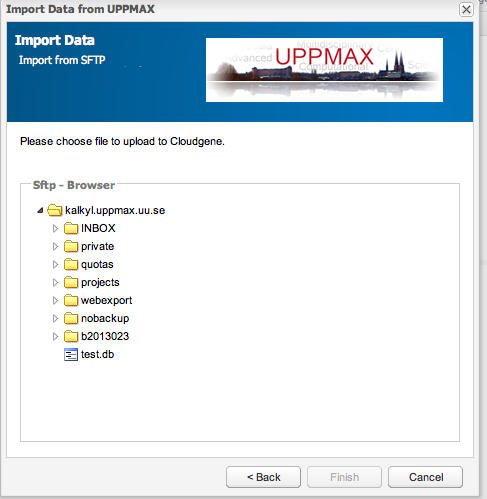
\includegraphics[width=\textwidth]{c.png}
		\subcaption{UPPMAX-adapted Cloudgene: browsing the users home folder}
	\end{subfigure}
 	\begin{subfigure}[b]{0.4\textwidth}
        	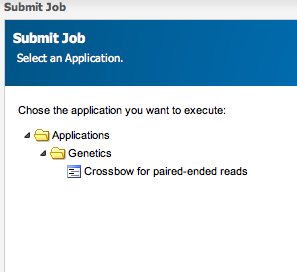
\includegraphics[width=\textwidth]{a.png}
		\subcaption{Cloudgene: selecting a job to run}
	\end{subfigure}
	\begin{subfigure}[b]{0.6\textwidth}
		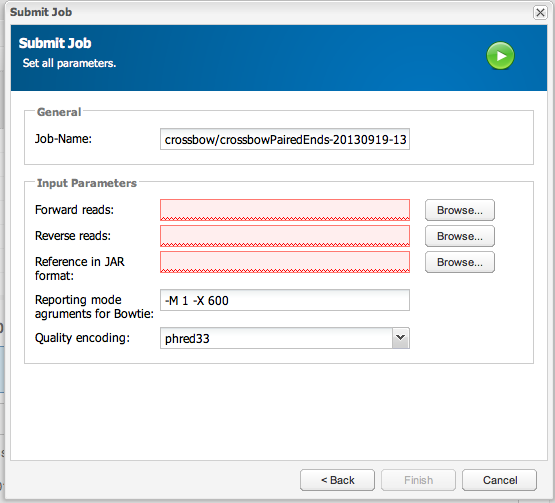
\includegraphics[width=\textwidth]{b.png}
		\subcaption{Cloudgene: specifying job parameters}
	\end{subfigure}
	\caption{An example of a job setup with the Cloudgene, a web-based GUI wrapper, providing a smooth user experience even for novice users.}
	\label{fig:fig4}
\end{figure}


\section{Conclusions}
\label{sectionV}

In this communication we brought together different approaches to analyze  the DNA-seq data in the bioinformatic study, in order to answer the question: which conditions a task should meet in order to make Hadoop a proper tool to use in favour of using HPC resources. 

To increase the performance of the existing Hadoop software, the modification to the preprocessing stage of the Crossbow software were suggested.  A state-of-art bash script was created to engage multiple nodes (up to 928 cores) in the HPC approach to align the Illumina-produced short reads with almost linear speed-ups.

We concentrated ourselves on the Hadoop  in the private cloud installation, Hadoop-in-the-Cloud, orchestrated by the OpenNebula. 
Picking the appropriate program settings we found out that DNA-seq dataset size larger than 100\,Gbases is suitable for Hadoop, with competitive  execution time compare to  that of HPC.
The scaling graphs (Figure~\ref{fig:fig1}) confirms the known fact for almost linear scalability of Hadoop.
The extrapolation to the infinite dataset size (Figure~\ref{fig:fig2}) revealed, that HPC, however, provides the results faster, given the same amount of resources, than the Hadoop-in-the-Cloud. 

Exploiting  the embarrassingly parallel nature of the short reads mapping we used custom state-of-art bash script to engage up to 58 nodes (928 cores) of the HPC2 cluster to  see the scaling relations between the ratio of the mapping time to the communication time as a function of a reciprocal number of nodes, Figure~\ref{fig:fig3}. 
Our results show that Hadoop with HDFS scales better than the network attached parallel storage commonly used in the HPC centers.
In addition we show  an example, how one can improve the performance of the HPC approach redefining the SLURM's default behaviour.


Finally, existing and easily transformed publically available web-based GUI, like Cloudgene~(Figure~\ref{fig:fig4}),  gives an opportunity to perform bioinformatic analysis on Hadoop for those who are not experts in Linux world.  Modular structure of Cloudgene gives cluster staff an easy way to adapt it for the specific needs.



\section{Acknowledge}
The computations were performed on resources provided by SNIC through Uppsala Multidisciplinary Center for Advanced Computational Science (UPPMAX) under Project p2013023.
We also greatly appreciate   Pontus Freyhult and Peter Ankerst{\aa}l at  UPPMAX for explaining the effective storage usage. Great job was done by Jonas Hagberg at BILS, Stockholm, Sweden, by the adaptation of the Cloudgene to the local UPPMAX needs.



\section{Supplementary material}

\subsection{Used datasets}

The datasets used in the paper are publicly available at:

I: \url{http://1001genomes.org/data/software/shoremap/shoremap\_2.0\\/data/reads/Schneeberger.2009/Schneeberger.2009.single\_end.gz}

II: \url{http://1001genomes.org/data/software/shoremap/shoremap\_2.0/data/reads/Galvao.2012/Galvao.2012.reads1.fq.gz, http://1001genomes.org/data/software/shoremap/shoremap\_2.0/data/reads/Galvao.2012/Galvao.2012.reads2.fq.gz}	

III: \url{ftp://ftp-trace.ncbi.nlm.nih.gov/sra/sra-instant/reads/ByRun/sra/SRR/SRR611/SRR611084//SRR611084.sra, ftp://ftp-trace.ncbi.nlm.nih.gov/sra/sra-instant/reads/ByRun/sra/SRR/SRR611/SRR611085//SRR611085.sra}

IV: artificial pair-ended dataset for {\it A.thaliana} created with the {\tt wgsim} program from the Samtools package.

V: \url{http://www.ncbi.nlm.nih.gov/sra/SRX148888}


\subsection{Reference genomes}
\begin{itemize}
\item TAIR10 for datasets II-IV \url{ftp://ftp.arabidopsis.org/home/tair/Sequences/whole\_chromosomes/*.fas}
\item TAIR8 for dataset I \url{ftp://ftp.arabidopsis.org/home/tair/Genes/TAIR8\_genome\_release/}
\item H.sapiens, NCBI v37 \url{ftp://ftp.ccb.jhu.edu/pub/data/bowtie\_indexes/h\_sapiens\_37\_asm.ebwt.zip}
\end{itemize}

\subsection{Description of computational facilities}

\begin{enumerate}
\item  HPC1:
The HPC analysis pipeline was run on a node from the Kalkyl~\cite{kalkyl} cluster, equipped with two quad-core processors Intel Xeon~5520 (clock frequency of 2.26\,GHz; 1\,MB L2 cache, 8\,MB L3 cache), 24\,GB of RAM and an Infiniband node-to-node network connection, and 10Gbit/s uplink. The data and reference genomes were read and written to a parallel shared storage system. 

\item 
HPC2:
Multinode short read mapping was performed on the Milou cluster\cite{milouCluster} , equipped with dual 8cores CPUs Intel Xeon E5-2660, ( 2.2 GHz, 2\,MB L2 cache, 20\,MB L3 cache.), 128\,GB of RAM, Infiniband node-to-node network connection, and 10Gbit/s uplink.

\item Storage: 
Gulo\cite{gulo} is a custom built Lustre 2.4 system using 8 HP nodes with MDS600 storage boxes and an additional node for metadata handling. In total, it provides roughly 1 PB of storage and is accessed with Lustre's own protocol. It supports data striping over multiple nodes and disk targets and can give a theoretical single file read performance of up to 80 Gbit per second.

\item Our main Hadoop test platform was deployed on the private cloud at UPPMAX, using the OpenNebula~\cite{opennebula} cloud management system. Each node in this deployment was equipped with dual quad-core CPUs (Intel Xeon 5420; clock frequency of 2.50GHz\,GHz; 12~MB L2 cache), 16~GB RAM, one 1~TB SATA disk and Gigabit Ethernet. The cluster was set up with Cloudera Hadoop Distribution version~2.0.0-cdh4.4.0~\cite{cloudera}.

\end{enumerate}

\bibliography{text1}
\bibliographystyle{unsrt}

\end{document}